\documentclass[handout]{beamer}
\setbeamertemplate{navigation symbols}{}
\usepackage[utf8x]{inputenc}
\usepackage[T1]{fontenc}
\usepackage{pgfplots}
\usepackage{siunitx}
\usepackage{graphicx}
\usepackage{booktabs}


\newlength\figureheight
\newlength\figurewidth


\usetheme{Montpellier}
%\usecolortheme{beaver}
%\usepackage{ngerman}
%\beamersetuncovermixins{\opaqueness<1>{25}}{\opaqueness<2->{15}}

%\setbeamercovered{invisible}
\begin{document}
\title{Adversarial examples}
%\subtitle{Analysis of Data from Monkey Cerebral Cortex}  
\author{Jan-Hendrik Plank, Jonas Dehning \& Philipp Höhne}
\date{\today} 
%\titlegraphic{\includegraphics[width=\textwidth,height=.5\textheight]{someimage}}


\begin{frame}
\titlepage
\end{frame} 

\begin{frame}
\frametitle{Table of Contents}
\tableofcontents
\end{frame} 

\section{Data sets}

\begin{frame}
\frametitle{The data sets} 
\begin{columns}[T]
\begin{column}{0.5\textwidth}
\centering
MNIST
\begin{figure}
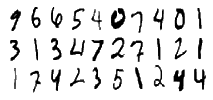
\includegraphics[width=0.7\linewidth]{./pictures/MNIST.png}
\end{figure}
\end{column}
\begin{column}{0.5\textwidth}
\centering
Dogs vs. Cats
\begin{figure}
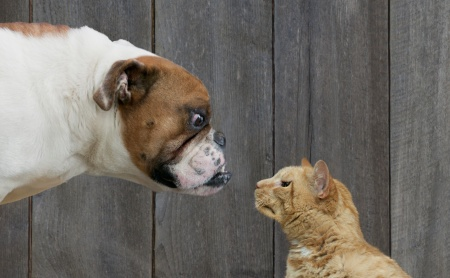
\includegraphics[width=0.7\linewidth]{./pictures/dogs_vs_cats.jpg}
\end{figure}
\end{column}
\end{columns}

\end{frame} 
%slide numbering
%videa scrambling, temporal receptor fields larger uri hasson
%summary slide
%changes of task

\begin{frame}
\frametitle{Networks}
\begin{itemize}
\item CNN
\end{itemize}
\begin{table}
\centering
\begin{tabular}{l c c} 
\toprule
Data set & Network structure & \# Layers \\ 
\midrule
MNIST & 5 CL - 2 FC & 7 \\  
Dogs vs. Cats & 11 CL - 3 FC & 14 \\
\bottomrule 
\end{tabular} 
\end{table}
\end{frame}

\section{Methods}

\begin{frame}
\frametitle{Finding adversarial examples: Gradient Method}

\begin{equation*}
\vec{\eta} = \epsilon \cdot \operatorname{sign} \left( \nabla_{\vec{x}} J_{loss} \big \vert_{\vec{x}} \right) 
\end{equation*}

\begin{align*}
\hspace{18em} &\vec{\eta}: \text{noise} \\
\hspace{18em} &\vec{x}: \text{picture} \\
\hspace{18em} &\epsilon \ll 1 
\end{align*}

\end{frame}

\begin{frame}
\frametitle{Finding adversarial examples: Minimizer}

Minimize over $\eta$:
\begin{align*}
\min_{\vec{\eta}} \left(\frac{1}{1 + \delta - p(\vec{x}+\vec{\eta})} + c \cdot \sigma(\vec{\eta}) \right) & \\
&\vec{\eta}: \text{noise} \\
&\vec{x}: \text{picture} \\
&p: \text{prediction} \\
&c: \text{a constant} \\
&\delta \ll 1 
\end{align*}

with constraint:
\begin{equation*}
\vec{x}+\vec{\eta}\in [0,1]^n
\end{equation*}


\end{frame}

\section{Visualization of adversarial examples}

\begin{frame}
\frametitle{MNIST adversarial examples I} 
\begin{figure}
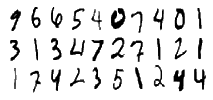
\includegraphics[width=0.9\linewidth]{./pictures/MNIST.png}
\end{figure}
\end{frame}

\begin{frame}
\frametitle{MNIST adversarial examples II} 
\begin{figure}
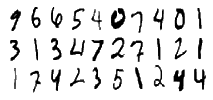
\includegraphics[width=0.9\linewidth]{./pictures/MNIST.png}
\end{figure}
\end{frame}

\begin{frame}
\frametitle{Dogs vs. Cats adversarial examples I} 
\begin{figure}
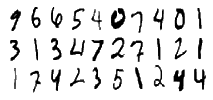
\includegraphics[width=0.9\linewidth]{./pictures/MNIST.png}
\end{figure}
\end{frame}

\begin{frame}
\frametitle{Dogs vs. Cats adversarial examples II} 
\begin{figure}
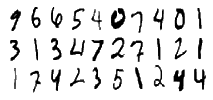
\includegraphics[width=0.9\linewidth]{./pictures/MNIST.png}
\end{figure}
\end{frame}



%\begin{frame}
%\frametitle{Adversarial examples}
%\begin{itemize}
%\item Small pertubations $\rightarrow$ false classification
%\end{itemize}
%\begin{figure}
%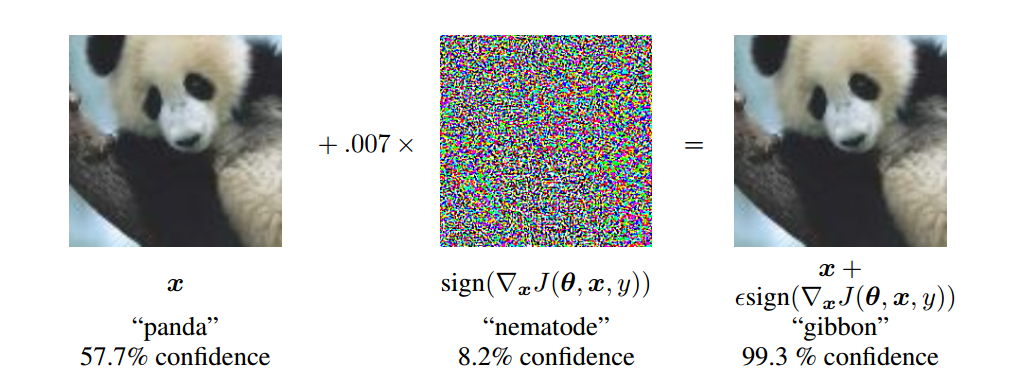
\includegraphics[width=0.9\linewidth]{./PandaGibbon}
%\end{figure}
%\begin{itemize}
%\item From Goodfellow et al. 2015
%\end{itemize}
%\end{frame}
%
%\begin{frame}
%\frametitle{Further ideas}
%\begin{itemize}
%\item improve network by training with the perturbed images
%\begin{itemize}
%\item improved kaggle score?
%\end{itemize}
%\item compare different datasets
%\item compare robustness of different networks
%\end{itemize}
%\end{frame}
%













\end{document}